\documentclass[11pt]{article}
	\usepackage[fleqn]{amsmath}
	\usepackage{float}
	\usepackage{caption}
	\usepackage{graphicx}
	\usepackage[margin=1in]{geometry}
	\usepackage{color}
	\title{Project 2 Report}
	\author{Group 29: Feiyu Zheng(fz114) \& Xueyang Chen(xc186)}
	\date{\today}
\begin{document}
	\maketitle
	\section*{1. How do we do feature extraction?}
		We use each single pixel in the graph as a feature, and the name/key for each feature is its location. If it is a white space, we assign the value of this feature to 0, otherwise 1.

	\section*{2. How do we implement each algorithm?}
		\subsection*{Naive Bayes:}
			\flushleft{}Since we need to use Bayes Rule equation to predict the probabilities of each outcome(label), we have to implement it in the coding. For Baye Rule, \\(\textcolor{red}{a}) \textcolor{blue}{probability of outcome(specific label) given a feature set of a sample} is equal to the product of (\textcolor{red}{b}) \textcolor{blue}{probability of outcome(specific label)} and (\textcolor{red}{c}) \textcolor{blue}{probability of this data given outcome is a specific label} divided by (\textcolor{red}{d}) \textcolor{blue}{the probability of the data}.\\
			\flushleft{}Because we only need to know which outcome(label) has the greatest probability, we compare the value of each outcome(label) for the same data(sample). Since (\textcolor{red}{d}) \textcolor{blue}{the probabilities of the data} are always the same, we just need to compare the value of (\textcolor{red}{b}) \textcolor{blue}{probability of outcome(specific label)} times (\textcolor{red}{c}) \textcolor{blue}{probability of this data given outcome is a specific label}.\\
			\flushleft{}Because multiplying many probabilities together often results in underflow, we will instead compute log probabilities.\\
			
			\flushleft{}For (\textcolor{red}{b}) \textcolor{blue}{probability of outcome(specific label)}, we use the number of samples with specific label divided by total number of samples. Then, calculate its log value.\\
			
			\flushleft{}For (\textcolor{red}{c}) \textcolor{blue}{probability of this data given outcome is a specific label}, it is the same as the product of (\textcolor{red}{e}) \textcolor{blue}{the probability of each feature given a specific outcome(label)}. We calculate each (\textcolor{red}{e}) \textcolor{blue}{probability of a single feature given a specific probability(label)}, and then multiply their log values.\\
			
			\flushleft{}For (\textcolor{red}{e}) \textcolor{blue}{probability of a single feature given a specific probability(label)},  we count the total times a specific feature has value 0 with a specific label, and divided by the total number of samples with this specific label. Since we only have two possible values for each feature(0 and 1), if a specific feature has value 1, then we use 1 minus the probability we have above to get the answer. Lastly, we convert the value to log value.\\
			
			\flushleft{}{}We sum all log values we get above to get our log probability of a specific label for a data. The label with greatest probability is our final prediction.\\
			
			\flushleft{}When we do the training process, we use a smoothing parameter \textcolor{blue}{k} to improve the accuracy of prediction. We have a set of 10 different \textcolor{blue}{k} values, and each iteration runs with one k value. After 10 iterations, we assign \textcolor{blue}{k} to the value with best accuracy.
		
		\subsection*{Perceptron:}
			\flushleft{}For all training data, we pick them one by one to do the following training process:
			\begin{itemize}
				\item[(1)]For each training data, we have A features vectors and B labels. Then we initialize the weight as a BxA matrix which contains small values (0.5 in our project). Multiplying the weight matrix by the features vectors will yield a vector that contains a value corresponding to each label. Among these values, we choose the label with the largest value as our prediction
				\item[(2)] We compare our prediction with the actual answer and take different actions depending on the comparison result.\\
				\begin{itemize}
					\item[(a)] If the label we predict is right, then we don’t modify the weight and jump to the next picture.
					\item[(b)] If the label we predict is not the same with the actual label,
					\begin{itemize}
						\item[(i)] we increase the weight value used for the real label if the current result for the real label is less than zero.
						\item[(ii)] we decrease the weight value used for the prediction label if the current result for that label is greater than zero.
					\end{itemize}
				\end{itemize}
				\item[(3)] We keep doing the above two steps until the algorithm reaches the iteration limits we predefined or there is no weight value change for all training data.
			\end{itemize}

	\section*{3. The learning curve for each case.}
		\begin{figure}[H]
			\centering
			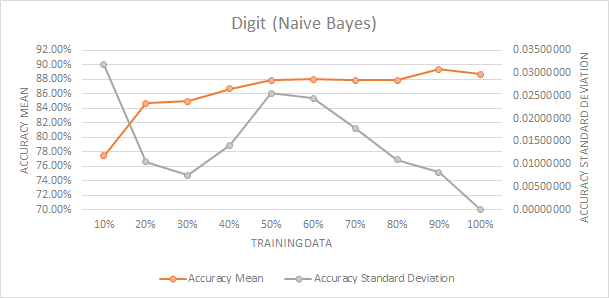
\includegraphics[scale=0.8]{Accuracy Digit (Naive Bayes).jpg}
			\caption{Accuracy of Using Naive Bayes on Digit Data}\label{fig:1}
		\end{figure}
		\begin{figure}[H]
			\centering
			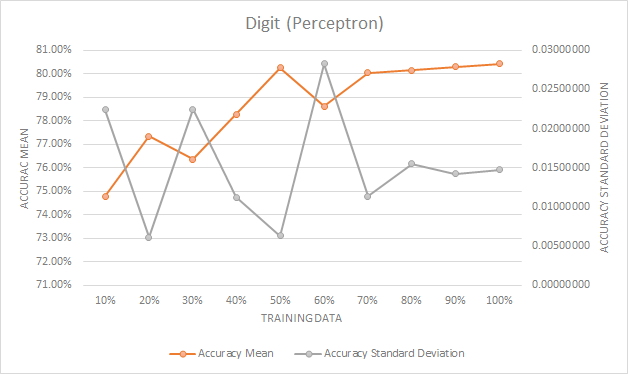
\includegraphics[scale=0.8]{Accuracy Digit (Perceptron).jpg}
			\caption{Accuracy of Using Perceptron on Digit Data}\label{fig:1}
		\end{figure}
		\begin{figure}[H]
			\centering
			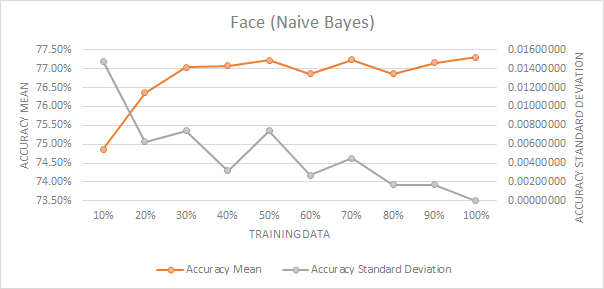
\includegraphics[scale=0.8]{Accuracy Face (Naive Bayes).jpg}
			\caption{Accuracy of Using Naive Bayes on Face Data}\label{fig:1}
		\end{figure}
		\begin{figure}[H]
			\centering
			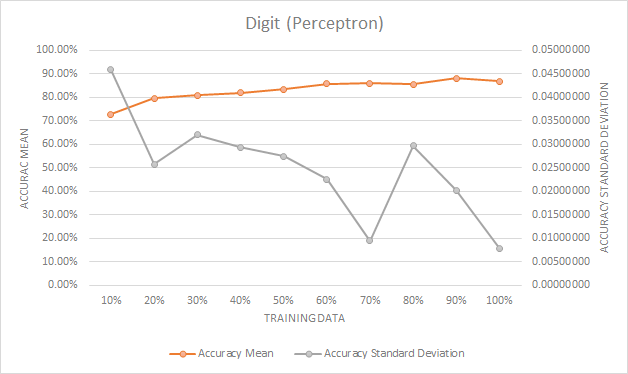
\includegraphics[scale=0.8]{Accuracy Face (Perceptron).jpg}
			\caption{Accuracy of Using Perceptron on Face Data}\label{fig:1}
		\end{figure}
		\flushleft{}As above Figure 1-4 show, we can see that the accuracy goes up as we are using more and more training data and we can also see a trend that the amount of data needed to increase the accuracy is increasing as the accuracy keeps increasing. As we are getting higher and higher accuracy, it’s harder and harder to increase the accuracy by adding more training data.
		\flushleft{}The following Figure 5-7 are the visualization of trained weight in the perceptron algorithm. With 100\% training data, the algorithm can already classify some labels by some points and know the general shape of a type of images.

		\begin{figure}[H]
			\centering
			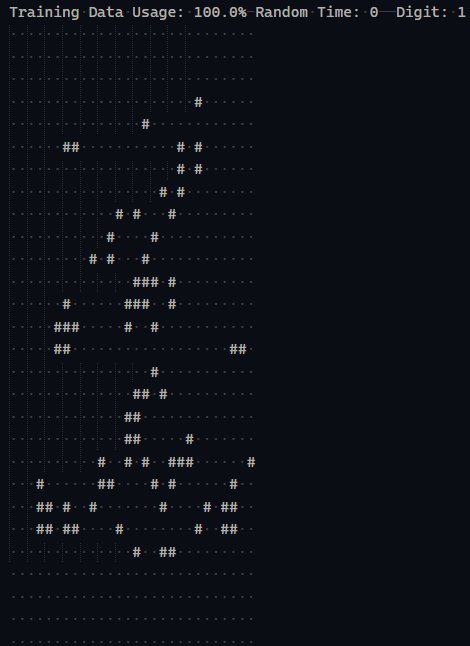
\includegraphics[scale=0.3]{Weight Visualization Digit 1.jpg}
			\caption{Perceptron Weight Visualization of Digit 1}\label{fig:1}
		\end{figure}
		\begin{figure}[H]
			\centering
			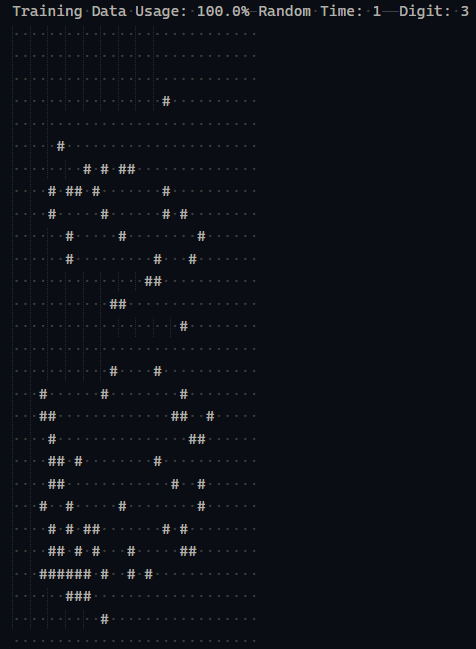
\includegraphics[scale=0.3]{Weight Visualization Digit 3.jpg}
			\caption{Perceptron Weight Visualization of Digit 3}\label{fig:1}
		\end{figure}
		\begin{figure}[H]
			\centering
			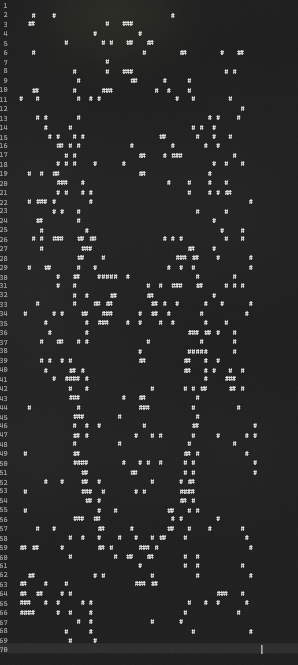
\includegraphics[scale=0.4]{Weight Visualization Face.jpg}
			\caption{Perceptron Weight Visualization of Face}\label{fig:1}
		\end{figure}

	\section*{4. Our observation on statistics.}
		\begin{figure}[H]
			\centering
			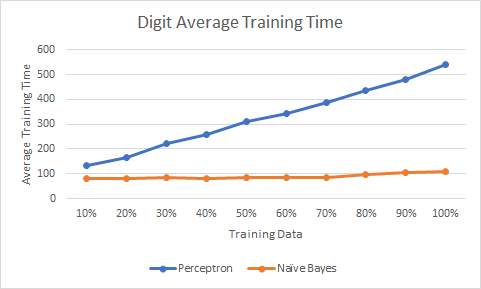
\includegraphics[scale=0.8]{Digit Average Training Time.jpg}
			\caption{Training Time of Perceptron and Naive Bayes When Using Digit Data}\label{fig:1}
		\end{figure}
		\begin{figure}[H]
			\centering
			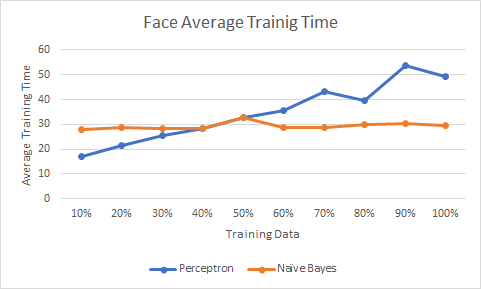
\includegraphics[scale=0.8]{Face Average Training Time.jpg}
			\caption{Training Time of Perceptron and Naive Bayes When Using Face Data}\label{fig:1}
		\end{figure}
		\flushleft{}Figure 8-9 show the time needed for training. We can see that as the number of training data gets larger and larger, the time needed for perceptron algorithms increases much faster than the naive bayes.
		\flushleft{}In Figure 1-4, the gray lines show the standard deviation as the number of data points increases during training. We can see a general pattern that as the size of training data increases, the prediction error is getting smaller and smaller and for Naive Bayes, the prediction error is always 0 when using 100\% training data.


	\section*{5. What can be improved in the future if it does not work well or does not have a high accuracy}
		\flushleft{}We can choose the better features which are more related to the result. For instance, the number of non-white space in a row or column, or the location of the farest gray space in each line.
		
		
\end{document}